\section{Additional Results}
\label{sec:supp_qualitative}

This section presents qualitative visualizations and quantitative ablations that complement the main paper's evaluation.
We first visualize the learned parameters, including per-vertex materials (Sec.~\ref{sec:qual_materials}), surface normals (Sec.~\ref{sec:qual_normals}), and antenna beam patterns (Sec.~\ref{sec:qual_beam}),to provide interpretability for the optimized representations.
We then ablate each component of the full model (Sec.~\ref{sec:ablation}) to quantify individual contributions and report runtime breakdowns (Sec.~\ref{sec:runtime}).

\subsection{Material Visualization}
\label{sec:qual_materials}

\begin{figure}[t]
  \centering
  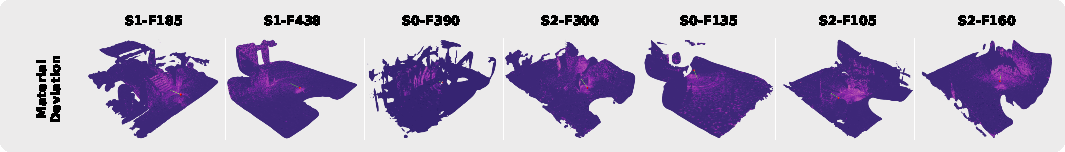
\includegraphics[width=\linewidth]{figs/materials_deviation_v1.pdf}
  \caption{Per-vertex material deviation from ITU-R P.2040 concrete defaults after optimization, shown across all seven scenes. Color encodes the normalized mean deviation across six physics parameters ($\varepsilon_r$, $\varepsilon_i$, $\sigma_h$, $\ell_c$, $\tau$, $d$) using the inferno colormap, where black = zero deviation (unchanged from defaults) and bright yellow = maximum deviation within each parameter's physical range. Log-scale parameters ($\varepsilon_i$, $\sigma_h$, $\ell_c$, $d$) are normalized in log-space; linear parameters ($\varepsilon_r$, $\tau$) in linear-space. Deviations concentrate on radar-visible surfaces and diminish in occluded or shadow regions.}
  \label{fig:3d_material}
\end{figure}

As shown in Fig.~\ref{fig:3d_material}, material deviations are
spatially correlated with radar visibility: surfaces under direct
illumination show the largest updates, while occluded regions retain
their ITU defaults. This pattern is consistent across all seven scenes
despite varying geometry and viewpoints.

\subsection{Surface Normal Visualization}
\label{sec:qual_normals}

\begin{figure}[t]
  \centering
  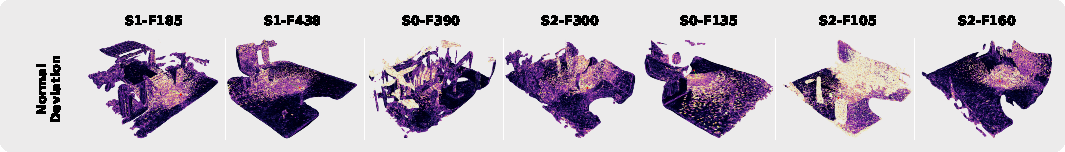
\includegraphics[width=\linewidth]{figs/normals_deviation_v1.pdf}
  \caption{Per-vertex angular deviation between initial (LiDAR-derived) and optimized surface normals across all seven scenes. Color encodes the absolute angle between initial and optimized normal vectors using the inferno colormap, where black = $0^{\circ}$ (no change) and bright yellow = $30^{\circ}$ or greater (clamped at $30^{\circ}$). Larger deviations appear primarily at mesh boundaries and on surfaces with irregular tessellation.}
  \label{fig:normals_deviation}
\end{figure}

\begin{figure}[t]
  \centering
  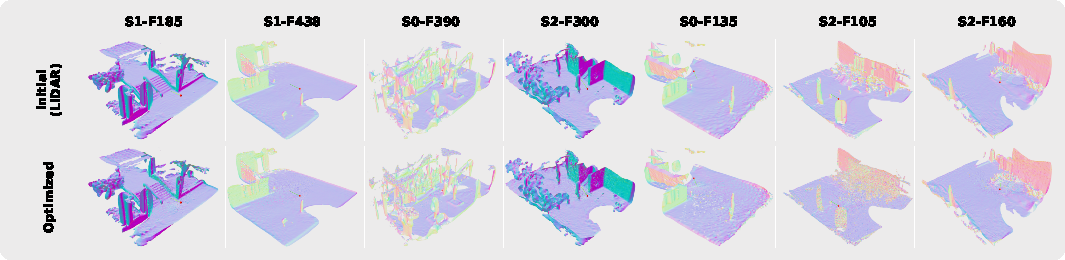
\includegraphics[width=\linewidth]{figs/normals_comparison_v1.pdf}
  \caption{World-space surface normal comparison across all seven scenes. Each vertex is colored by its unit normal direction mapped to RGB (X$\to$R, Y$\to$G, Z$\to$B; value range $[-1,1] \to [0,1]$). Top row (``Initial''): normals computed from the Poisson-reconstructed LiDAR mesh. Bottom row (``Optimized''): normals after joint optimization. Differences between rows show where surface orientations changed during optimization; changes are most apparent at mesh boundaries and on large planar surfaces where Poisson reconstruction artifacts are common.}
  \label{fig:normals}
\end{figure}

Figure~\ref{fig:normals_deviation} shows that angular deviations are spatially concentrated at mesh boundaries, thin structures, and regions with irregular tessellation, all of which are known failure modes of Poisson surface reconstruction from sparse LiDAR returns. Mean angular deviations range from $4^{\circ}$ to $13^{\circ}$ across the seven scenes. Figure~\ref{fig:normals} provides the corresponding world-space normal comparison: large planar regions (walls, ground) remain largely unchanged, while edges and thin features show visible reorientation. This spatial pattern indicates that normal optimization corrects tessellation artifacts rather than overfitting to measurement noise.

\subsection{Antenna Beam Pattern Visualization}
\label{sec:qual_beam}

\begin{figure}[t]
  \centering
  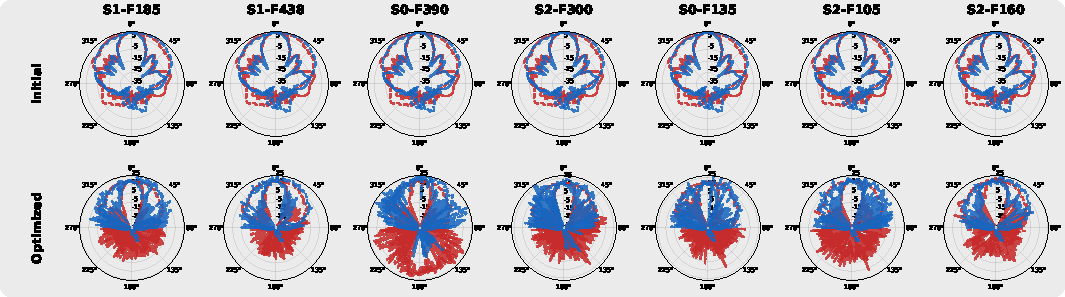
\includegraphics[width=\linewidth]{figs/beam_patterns_comparison_v1.pdf}
  \caption{Antenna beam pattern comparison across all seven scenes (polar plots, dB scale). Each plot shows four curves: TX elevation (red solid), TX azimuth (red dashed), RX elevation (blue solid), and RX azimuth (blue dashed). Top row (``Initial''): reference patterns shared across all scenes. Bottom row (``Optimized''): per-scene optimized patterns. Optimization adjusts main-lobe gain and sidelobe structure to compensate for calibration uncertainty in the reference antenna data. Per-scene variation in the optimized patterns is expected, as each scene compensates independently for calibration uncertainty. All values floored at the initial pattern minimum ($-32$\,dB).}
  \label{fig:beam_patterns}
\end{figure}

As shown in Fig.~\ref{fig:beam_patterns}, the optimized beam patterns retain the main-lobe beamwidths of the initial reference patterns for both TX and RX elements across elevation and azimuth, while adjusting absolute gain levels. Per-scene variation in the optimized patterns reflects independent compensation for calibration uncertainty. The consistent preservation of main-lobe structure across all seven scenes supports the interpretation that pattern optimization primarily refines gain calibration rather than learning physically implausible beam~shapes.


\FloatBarrier
\subsection{Ablation Studies}
\label{sec:ablation}

\begin{table}[ht!]
\caption{Component ablation averaged over seven training scenes (500
iterations each). Each row disables one component from the full mmIR
model. Best per-column in \textbf{bold}.}
\centering
\begin{tabular}{lcccc}
\toprule
\textbf{Configuration} & \textbf{Corr $\uparrow$} & \textbf{PSNR $\uparrow$} & \textbf{SSIM $\uparrow$} & \textbf{RMSE $\downarrow$} \\
\midrule
Full model              & 0.919 & 37.6 & 0.902 & 0.014 \\
\midrule
w/o diffraction         & 0.910 & 37.4 & 0.896 & 0.014 \\
w/o SMS                 & 0.915 & 37.8 & 0.898 & 0.014 \\
w/o multi-bounce        & \textbf{0.936} & \textbf{38.7} & \textbf{0.920} & \textbf{0.012} \\
w/o normal optim.       & 0.919 & 37.4 & 0.909 & 0.014 \\
w/o pattern optim.      & 0.885 & 36.6 & 0.882 & 0.015 \\
w/o error-map init      & 0.909 & 37.4 & 0.895 & 0.014 \\
\bottomrule
\end{tabular}
\label{tab:ablation}
\end{table}


We ablate each component by disabling it from the full model and
retraining on all seven scenes for 500 iterations
(Table~\ref{tab:ablation}). We group ablations into three categories:
rendering transport, optimization targets, and initialization.

\paragraph{Rendering transport.}
Disabling \emph{diffraction} degrades RA correlation ($0.919 \to 0.910$, $-1.0\%$), indicating that edge-diffracted energy
contributes in outdoor scenes with building edges, fences,
and vehicle contours.
%
Disabling \emph{SMS} has a marginal effect on RA metrics
($0.919 \to 0.915$), consistent with the predominantly rough surface
scattering expected at 77\,GHz for outdoor building materials;
SMS primarily benefits scenes with smooth metallic
surfaces (e.g., vehicle panels), which constitute a small fraction of
the total scattering area.
%
Restricting propagation to \emph{single-bounce} slightly improves RA
correlation ($0.919 \to 0.936$) and RMSE
($0.014 \to 0.012$). This suggests that higher-order bounces
introduce Monte Carlo variance at the current sample budget that
slightly degrades metrics, though indirect paths (e.g., ground--wall or
wall--vehicle interactions) contribute measurable energy in the
captured data.

\paragraph{Optimization targets.}
Disabling \emph{antenna pattern optimization} reduces PSNR by
1.0\,dB ($37.6 \to 36.6$) and degrades RA correlation
($0.919 \to 0.885$, $-3.7\%$), indicating that jointly learning beam patterns
compensates for calibration uncertainty in the initial reference antenna
data. As shown in Fig.~\ref{fig:beam_patterns}, the optimized patterns
retain the main-lobe structure and beamwidths of the initial reference
patterns for both TX and RX elements across elevation and azimuth,
indicating that optimization refines gain calibration while preserving
the physical beam structure. The consistent main-lobe preservation
across all seven scenes is consistent with the observation that
disabling pattern optimization primarily degrades PSNR (absolute power
calibration) rather than correlation (spatial structure).
%
Freezing \emph{surface normals} at their LiDAR-derived values has
negligible effect on RA correlation ($0.919 \to 0.919$), while slightly
improving SSIM ($0.902 \to 0.909$). As visualized in
Figs.~\ref{fig:normals_deviation} and~\ref{fig:normals}, normal
optimization concentrates adjustments at mesh boundaries and thin
structures (known failure modes of Poisson surface
reconstruction), with mean angular deviation of $4$--$13^{\circ}$
across scenes, while leaving large planar regions largely unchanged.
This spatial pattern suggests that normal optimization targets
tessellation artifacts rather than overfitting to measurement noise.

\paragraph{Initialization.}
Disabling \emph{error-map initialization} has marginal effect on
final metrics ($0.919 \to 0.909$), indicating that 500 gradient
iterations are sufficient to largely recover from uniform material
initialization. The benefit of error-map seeding is faster early
convergence rather than improved final quality.

\FloatBarrier
\subsection{Runtime}
\label{sec:runtime}

Table~\ref{tab:runtime} reports the runtime breakdown for our pipeline and the Sionna-RT baseline on scene S0F135 ($\sim$72K vertices) using a single NVIDIA RTX 4090 GPU (24\,GB).
Per-scene preprocessing---LiDAR aggregation, Poisson meshing, and radar--LiDAR alignment---is a one-time cost shared by both methods.
During training, our forward render averages 0.65\,s per iteration, roughly $4.5\times$ faster than Sionna-RT's 2.93\,s, owing to our Taichi-based SBR kernel and cached specular-path reuse.
The AD backward pass adds only 0.10\,s.
Including gradient clipping, the Adam optimizer step, and metric computation, the total per-iteration cost is 1.32\,s, enabling 500 iterations in $\sim$11\,min wall-clock time.
At inference, rendering the full dense virtual array (10,000 elements) and computing the RAE FFT takes 6.4\,s per scene.

\begin{table}[ht!]
\centering
\caption{Runtime comparison and breakdown on a single NVIDIA RTX 4090 GPU (24\,GB). Training times are averaged over 500 iterations (mmIR) and 150 iterations (Sionna-RT) on scene S0F135 ($\sim$72K vertices), excluding the first 5 iterations (JIT compilation warmup).}
\label{tab:runtime}
\begin{tabular}{lcc}
\toprule
\textbf{Stage} & \textbf{mmIR (Ours)} & \textbf{Sionna-RT} \\
\midrule
\multicolumn{3}{l}{\emph{Per-scene preprocessing (one-time)}} \\
\quad LiDAR aggregation \& meshing & \multicolumn{2}{c}{144\,s} \\
\quad LiDAR--radar alignment & \multicolumn{2}{c}{2.2\,s} \\
\midrule
\multicolumn{3}{l}{\emph{Training (per iteration, mean $\pm$ std)}} \\
\quad Forward render & 0.65\,s & 2.93\,s \\
\quad AD backward + grad.\ extraction & 0.10\,s & 0.35\,s \\
\quad Grad.\ clipping + optimizer + metrics & 0.57\,s & -- \\
\quad Total per iteration & 1.32 $\pm$ 0.02\,s & 3.28 $\pm$ 0.46\,s \\
\midrule
\multicolumn{3}{l}{\emph{Training (total)}} \\
\quad Total wall-clock & 11.0\,min & 8.2\,min \\
\quad Iterations & 500 & 150 \\
\midrule
\multicolumn{3}{l}{\emph{Inference (one-time per scene)}} \\
\quad Dense array ADC rendering & \multicolumn{2}{c}{6.2\,s} \\
\quad RAE FFT + point cloud & \multicolumn{2}{c}{0.2\,s} \\
\bottomrule
\end{tabular}
\end{table}
